
\documentclass[11pt,a4paper]{article}

% -----------------------------
% PACKAGES
% -----------------------------
\usepackage[margin=1in]{geometry}
\usepackage{parskip}
\usepackage{lmodern}
\usepackage{hyperref}
\usepackage{titlesec}
\usepackage{tikz}
\usepackage{pgfplots}
\pgfplotsset{compat=1.18}

% Section formatting
\titleformat{\section}{\Large\bfseries}{\thesection}{1em}{}
\titleformat{\subsection}{\large\bfseries}{\thesubsection}{1em}{}

% -----------------------------
% DOCUMENT
% -----------------------------
\begin{document}

% Cover block (simple, GitHub PDF-friendly)
\begin{center}
    {\LARGE \textbf{Lock The System}}\\[0.3cm]
    {\Large A Structural Liquidity Framework for Intraday XAU/USD}\\[0.6cm]
    {\large Valentino De Vivo — Independent Research Framework (2026)}\\[0.4cm]
\end{center}
\vspace{0.6cm}

\begin{abstract}
This executive, CV-ready summary presents a structural liquidity framework for intraday XAU/USD. The model evaluates directional bias only when four dimensions—structure, liquidity, time, and volume—converge. The objective is to reduce discretionary variability through a hierarchical, conditional alignment process. Diagrams and a conceptual session-volatility plot are embedded to illustrate the mechanics.
\end{abstract}

\section{Framework Overview}
Intraday price action often appears noisy when viewed via isolated signals. XAU/USD exhibits recurring sequences around structural transitions, liquidity interaction, and session-driven volatility. This framework imposes a layered decision architecture that prioritizes omission unless conditions align.

\section{Core Model Dimensions}
\subsection{Structure}
External structure defines directional context via major swing sequences; internal structure captures short-term corrections. The separation avoids misclassifying retracements as reversals.

\subsection{Liquidity}
Prior highs/lows and consolidation boundaries concentrate orders. Interaction with these zones provides context but requires confirmed displacement to infer direction.

\subsection{Time}
Volatility and participation vary by session. Asian trading is typically range-bound; European and U.S. sessions more often generate displacement. Time acts as a reliability filter rather than a predictor.

\subsection{Volume}
Volume validates movement by comparing effort and result. Rising volume during expansion supports continuation; high volume with limited progress implies absorption; declining volume during retracement suggests corrective behaviour.

\section{Structural Hierarchy Model}
The hierarchy proceeds through: (1) external structure, (2) internal structure, (3) liquidity interaction, and (4) structural displacement. The TikZ diagram below places the components in sequence.

\begin{center}
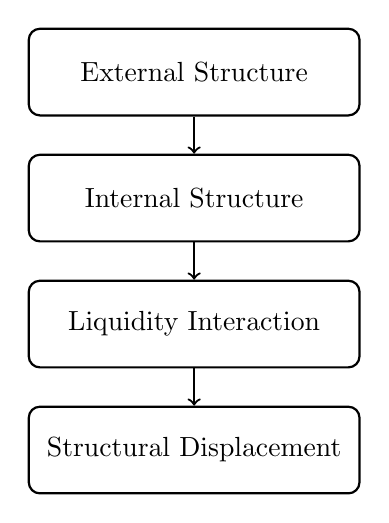
\begin{tikzpicture}[node distance=1.6cm]
  \tikzstyle{box}=[rectangle, draw, rounded corners, minimum width=4.2cm, minimum height=1.1cm, thick]
  \node[box] (ext) {External Structure};
  \node[box, below of=ext] (int) {Internal Structure};
  \node[box, below of=int] (liq) {Liquidity Interaction};
  \node[box, below of=liq] (disp) {Structural Displacement};
  \draw[->, thick] (ext) -- (int);
  \draw[->, thick] (int) -- (liq);
  \draw[->, thick] (liq) -- (disp);
\end{tikzpicture}
\end{center}

\section{Time-Based Volatility Model}
Session timing acts as an activation filter. The PGFPlots figure below visualizes a conceptual volatility profile across major sessions.

\begin{center}
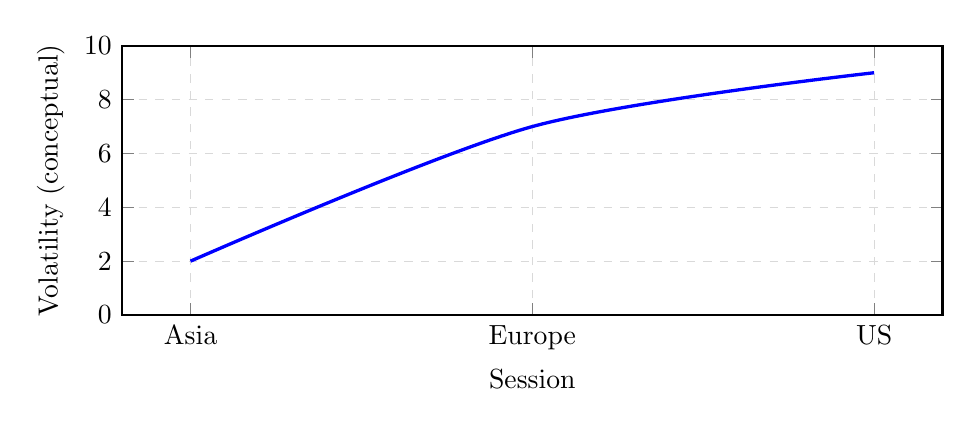
\begin{tikzpicture}
\begin{axis}[
  xlabel=Session,
  ylabel=Volatility (conceptual),
  xtick={1,2,3},
  xticklabels={Asia, Europe, US},
  ymin=0, ymax=10,
  width=12cm, height=5cm,
  grid=major, grid style={dashed, gray!30},
  thick
]
\addplot[smooth, very thick, blue] coordinates {(1,2) (2,7) (3,9)};
\end{axis}
\end{tikzpicture}
\end{center}

\section{Volume Integration}
Volume helps distinguish continuation (expansion with rising volume), absorption (high volume, limited progress), and corrective phases (declining volume in retracement). Volume is never treated as a standalone signal.

\section{Conditional Alignment Model}
Execution is considered only when five conditions align: (1) external bias, (2) liquidity interaction, (3) confirmed displacement, (4) favourable session timing, and (5) supportive volume behaviour. When any layer fails, the default stance is non-participation.

\section{Model Limitations}
The framework is conceptual and currently tailored to XAU/USD. Structural identification can be partially discretionary without rule encoding, and macro shocks may invalidate conditions. Future work includes statistical validation, rule parametrization, and automation.

\end{document}
